\title{2016 年高考数学 全国III卷-文科}
\date{}
\maketitle

\section*{一、选择题}
共 12 小题，每小题 5 分，满分 60 分。

\begin{question}[points=5]
设集合 $A=\{0, 2, 4, 6, 8, 10\}$, $B=\{4, 8\}$, 则 $\complement_AB=$ ( )
\begin{choices}
  \item $\{4, 8\}$
  \item $\{0, 2, 6\}$
  \item $\{0, 2, 6, 10\}$
  \item $\{0, 2, 4, 6, 8, 10\}$
\end{choices}
\begin{solution}
\textbf{答案：}$\{0, 2, 6, 10\}$

\textbf{分析：}根据全集 $A$ 求出 $B$ 的补集即可.

\textbf{详解：}集合 $A=\{0, 2, 4, 6, 8, 10\}$, $B=\{4, 8\}$, 则 $\complement_AB=\{0, 2, 6, 10\}$. 故选 C.
\end{solution}
\end{question}

\begin{question}[points=5]
若 $z=4+3i$, 则 $\dfrac{\overline{z}}{|z|}=$ ( )
\begin{choices}
  \item $1$
  \item $-1$
  \item $\dfrac{4}{5}+\dfrac{3}{5}i$
  \item $\dfrac{4}{5}-\dfrac{3}{5}i$
\end{choices}
\begin{solution}
\textbf{答案：}$\dfrac{4}{5}-\dfrac{3}{5}i$

\textbf{分析：}利用复数的除法以及复数的模化简求解即可.

\textbf{详解：}$z=4+3i$, 则 $\dfrac{\overline{z}}{|z|}=\dfrac{4-3i}{\sqrt{4^2+3^2}}=\dfrac{4-3i}{5}=\dfrac{4}{5}-\dfrac{3}{5}i$. 故选 D.
\end{solution}
\end{question}

\begin{question}[points=5]
已知向量 $\overrightarrow{BA}=(\dfrac{1}{2},\dfrac{\sqrt{3}}{2})$, $\overrightarrow{BC}=(\dfrac{\sqrt{3}}{2},\dfrac{1}{2})$, 则 $\angle ABC=$ ( )
\begin{choices}
  \item $30^{\circ}$
  \item $45^{\circ}$
  \item $60^{\circ}$
  \item $120^{\circ}$
\end{choices}
\begin{solution}
\textbf{答案：}$30^{\circ}$

\textbf{分析：}根据向量 $\overrightarrow{BA}$ 和 $\overrightarrow{BC}$ 的坐标求出 $\overrightarrow{BA}\cdot\overrightarrow{BC}$ 及 $|\overrightarrow{BA}|,|\overrightarrow{BC}|$ 的值, 从而根据向量夹角余弦公式即可求出 $\cos\angle ABC$ 的值, 根据 $\angle ABC$ 的范围便可得出 $\angle ABC$ 的值.

\textbf{详解：}$\overrightarrow{BA}=(\dfrac{1}{2},\dfrac{\sqrt{3}}{2})$, $\overrightarrow{BC}=(\dfrac{\sqrt{3}}{2},\dfrac{1}{2})$; 则 $\overrightarrow{BA}\cdot\overrightarrow{BC}=\dfrac{1}{2}\cdot\dfrac{\sqrt{3}}{2}+\dfrac{\sqrt{3}}{2}\cdot\dfrac{1}{2}=\dfrac{\sqrt{3}}{2}$, $|\overrightarrow{BA}|=1$, $|\overrightarrow{BC}|=1$; 所以 $\cos\angle ABC=\dfrac{\overrightarrow{BA}\cdot\overrightarrow{BC}}{|\overrightarrow{BA}||\overrightarrow{BC}|}=\dfrac{\sqrt{3}}{2}$; 又 $0^{\circ}\le\angle ABC\le180^{\circ}$; 所以 $\angle ABC=30^{\circ}$. 故选 A.
\end{solution}
\end{question}

\begin{question}[points=5]
某旅游城市为向游客介绍本地的气温情况, 绘制了一年中各月平均最高气温和平均最低气温的雷达图, 图中 $A$ 点表示十月的平均最高气温约为 $15^{\circ}C$, $B$ 点表示四月的平均最低气温约为 $5^{\circ}C$, 下面叙述不正确的是 ( )

\begin{center}
  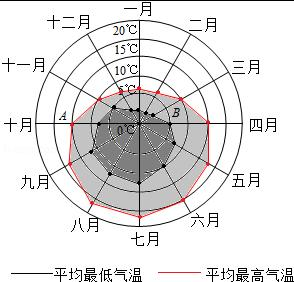
\includegraphics[width=.38\linewidth]{question-4-1.jpg}
\end{center}
\begin{choices}
  \item 各月的平均最低气温都在 $0^{\circ}C$ 以上
  \item 七月的平均温差比一月的平均温差大
  \item 三月和十一月的平均最高气温基本相同
  \item 平均最高气温高于 $20^{\circ}C$ 的月份有 $5$ 个
\end{choices}
\begin{solution}
\textbf{答案：}平均最高气温高于 $20^{\circ}C$ 的月份有 $5$ 个

\textbf{分析：}根据平均最高气温和平均最低气温的雷达图进行推理判断即可.

\textbf{详解：}A. 由雷达图知各月的平均最低气温都在 $0^{\circ}C$ 以上, 正确. B. 七月的平均温差大约在 $10^{\circ}$ 左右, 一月的平均温差在 $5^{\circ}$ 左右, 故七月的平均温差比一月的平均温差大, 正确. C. 三月和十一月的平均最高气温基本相同, 都为 $10^{\circ}$, 正确. D. 平均最高气温高于 $20^{\circ}C$ 的月份有 $7,8$ 两个月, 故 D 错误. 故选 D.
\end{solution}
\end{question}

\begin{question}[points=5]
小敏打开计算机时, 忘记了开机密码的前两位, 只记得第一位是 $M$, $I$, $N$ 中的一个字母, 第二位是 $1$, $2$, $3$, $4$, $5$ 中的一个数字, 则小敏输入一次密码能够成功开机的概率是 ( )
\begin{choices}
  \item $\dfrac{1}{15}$
  \item $\dfrac{1}{8}$
  \item $\dfrac{1}{15}$
  \item $\dfrac{1}{30}$
\end{choices}
\begin{solution}
\textbf{答案：}$\dfrac{1}{15}$

\textbf{分析：}列举出从 $M$, $I$, $N$ 中任取一个字母, 再从 $1$, $2$, $3$, $4$, $5$ 中任取一个数字的基本事件数, 然后由随机事件发生的概率得答案.

\textbf{详解：}从 $M$, $I$, $N$ 中任取一个字母, 再从 $1$, $2$, $3$, $4$, $5$ 中任取一个数字, 取法总数为 $(M,1),(M,2),(M,3),(M,4),(M,5),(I,1),(I,2),(I,3),(I,4),(I,5),(N,1),(N,2),(N,3),(N,4),(N,5)$ 共 $15$ 种. 其中只有一个是小敏的密码前两位. 由随机事件发生的概率可得, 小敏输入一次密码能够成功开机的概率是 $\dfrac{1}{15}$. 故选 C.
\end{solution}
\end{question}

\begin{question}[points=5]
若 $\tan\theta=\dfrac{1}{3}$, 则 $\cos2\theta=$ ( )
\begin{choices}
  \item $\dfrac{4}{5}$
  \item $\dfrac{1}{5}$
  \item $\dfrac{1}{5}$
  \item $\dfrac{3}{5}$
\end{choices}
\begin{solution}
\textbf{答案：}$\dfrac{4}{5}$

\textbf{分析：}原式利用二倍角的余弦函数公式变形, 再利用同角三角函数间的基本关系化简, 将 $\tan\theta$ 的值代入计算即可求出值.

\textbf{详解：}$\tan\theta=\dfrac{1}{3}$, 则 $\cos2\theta=2\cos^2\theta-1=\dfrac{2}{1+\tan^2\theta}-1=\dfrac{2}{1+\frac{1}{9}}-1=\dfrac{2}{\frac{10}{9}}-1=\dfrac{18}{10}-1=\dfrac{8}{10}=\dfrac{4}{5}$. 故选 D.
\end{solution}
\end{question}

\begin{question}[points=5]
已知 $a=2^{\frac{4}{3}}$, $b=4^{\frac{2}{5}}$, $c=25^{\frac{1}{3}}$, 则 ( )
\begin{choices}
  \item $b<a<c$
  \item $a<b<c$
  \item $b<c<a$
  \item $c<a<b$
\end{choices}
\begin{solution}
\textbf{答案：}$b<a<c$

\textbf{分析：}$b=4^{\frac{2}{5}}=(2^2)^{\frac{2}{5}}=2^{\frac{4}{5}}$, $c=25^{\frac{1}{3}}=(5^2)^{\frac{1}{3}}=5^{\frac{2}{3}}$, 结合幂函数的单调性, 可比较 $a,b,c$.

\textbf{详解：}$a=2^{\frac{4}{3}}$, $b=2^{\frac{4}{5}}$, $c=5^{\frac{2}{3}}$, 由幂函数 $y=x^{\frac{4}{3}}$ 在 $(0,+\infty)$ 上递增, 得 $2^{\frac{4}{5}}<2^{\frac{4}{3}}<3^{\frac{4}{3}}$, 又 $3^{\frac{4}{3}}=(3^4)^{\frac{1}{3}}=81^{\frac{1}{3}}$, $c=5^{\frac{2}{3}}=(5^2)^{\frac{1}{3}}=25^{\frac{1}{3}}$, 因为 $81>25$, 所以 $3^{\frac{4}{3}}>c$, 故 $b<a<c$. 故选 A.
\end{solution}
\end{question}

\begin{question}[points=5]
执行如图程序框图, 如果输入的 $a=4$, $b=6$, 那么输出的 $n=$ ( )

\begin{center}
  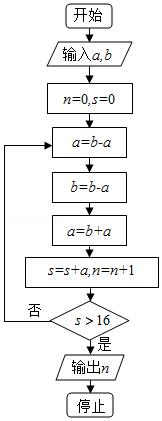
\includegraphics[width=.38\linewidth]{question-8-1.jpg}
\end{center}
\begin{choices}
  \item $3$
  \item $4$
  \item $5$
  \item $6$
\end{choices}
\begin{solution}
\textbf{答案：}$4$

\textbf{分析：}模拟执行程序, 根据赋值语句的功能依次写出每次循环得到的 $a,b,s,n$ 的值, 当 $s=20$ 时满足条件 $s>16$, 退出循环, 输出 $n$ 的值为 $4$.

\textbf{详解：}模拟执行程序, 可得 $a=4,b=6,n=0,s=0$; 执行循环体, $a=2,b=4,a=6,s=6,n=1$; 不满足条件 $s>16$, 执行循环体, $a=-2,b=6,a=4,s=10,n=2$; 不满足条件 $s>16$, 执行循环体, $a=2,b=4,a=6,s=16,n=3$; 不满足条件 $s>16$, 执行循环体, $a=-2,b=6,a=4,s=20,n=4$; 满足条件 $s>16$, 退出循环, 输出 $n$ 的值为 $4$. 故选 B.
\end{solution}
\end{question}

\begin{question}[points=5]
在 $\triangle ABC$ 中, $B=\dfrac{\pi}{4}$, $BC$ 边上的高等于 $\dfrac{1}{3}BC$, 则 $\sin A=$ ( )
\begin{choices}
  \item $\dfrac{3}{10}$
  \item $\dfrac{\sqrt{10}}{10}$
  \item $\dfrac{\sqrt{5}}{5}$
  \item $\dfrac{3\sqrt{10}}{10}$
\end{choices}
\begin{solution}
\textbf{答案：}$\dfrac{3\sqrt{10}}{10}$

\textbf{分析：}由已知, 结合勾股定理和余弦定理, 求出 $AB$, $AC$, 再由三角形面积公式, 可得 $\sin A$.

\textbf{详解：}在 $\triangle ABC$ 中, $B=\dfrac{\pi}{4}$, $BC$ 边上的高等于 $\dfrac{1}{3}BC$, 所以 $AB=\dfrac{\sqrt{2}}{3}BC$. 由余弦定理 $AC^2=AB^2+BC^2-2\cdot AB\cdot BC\cdot\cos B=\dfrac{2}{9}BC^2+BC^2-2\cdot\dfrac{\sqrt{2}}{3}BC\cdot BC\cdot\dfrac{\sqrt{2}}{2}=\dfrac{2}{9}BC^2+BC^2-\dfrac{2}{3}BC^2=\dfrac{5}{9}BC^2$, 故 $AC=\dfrac{\sqrt{5}}{3}BC$. 由面积公式 $\dfrac{1}{2}\cdot BC\cdot\dfrac{1}{3}BC=\dfrac{1}{2}\cdot AB\cdot AC\cdot\sin A$, 即 $\dfrac{1}{6}BC^2=\dfrac{1}{2}\cdot\dfrac{\sqrt{2}}{3}BC\cdot\dfrac{\sqrt{5}}{3}BC\cdot\sin A$, 解得 $\sin A=\dfrac{3\sqrt{10}}{10}$. 故选 D.
\end{solution}
\end{question}

\begin{question}[points=5]
如图, 网格纸上小正方形的边长为 $1$, 粗实线画出的是某多面体的三视图, 则该多面体的表面积为 ( )
\begin{choices}
  \item $18+36\sqrt{5}$
  \item $54+18\sqrt{5}$
  \item $90$
  \item $81$
\end{choices}
\begin{solution}
\textbf{答案：}$54+18\sqrt{5}$

\textbf{分析：}由已知中的三视图可得: 该几何体是一个以主视图为底面的直四棱柱, 进而得到答案.

\textbf{详解：}由已知中的三视图可得: 该几何体是一个以主视图为底面的直四棱柱, 其底面面积为 $3\times6=18$, 侧面的面积为 $(3\times3+3\times\sqrt{5})\times2=18+18\sqrt{5}$, 故棱柱的表面积为 $18\times2+18+18\sqrt{5}=54+18\sqrt{5}$. 故选 B.
\end{solution}
\end{question}

\begin{question}[points=5]
在封闭的直三棱柱 $ABC-A_1B_1C_1$ 内有一个体积为 $V$ 的球, 若 $AB\perp BC$, $AB=6$, $BC=8$, $AA_1=3$, 则 $V$ 的最大值是 ( )
\begin{choices}
  \item $4\pi$
  \item $\dfrac{9\pi}{2}$
  \item $6\pi$
  \item $\dfrac{32\pi}{3}$
\end{choices}
\begin{solution}
\textbf{答案：}$\dfrac{9\pi}{2}$

\textbf{分析：}根据已知可得直三棱柱 $ABC-A_1B_1C_1$ 的内切球半径为 $\dfrac{3}{2}$, 代入球的体积公式, 可得答案.

\textbf{详解：}$AB\perp BC$, $AB=6$, $BC=8$, 所以 $AC=10$. 故三角形 $ABC$ 的内切圆半径 $r=\dfrac{6+8-10}{2}=2$. 又 $AA_1=3$, 故直三棱柱 $ABC-A_1B_1C_1$ 的内切球半径为 $\dfrac{3}{2}$. 此时 $V$ 的最大值 $\dfrac{4}{3}\pi\left(\dfrac{3}{2}\right)^3=\dfrac{9\pi}{2}$. 故选 B.
\end{solution}
\end{question}

\begin{question}[points=5]
已知 $O$ 为坐标原点, $F$ 是椭圆 $C:\dfrac{x^2}{a^2}+\dfrac{y^2}{b^2}=1$

$(a>b>0)$ 的左焦点, $A$, $B$ 分别为 $C$ 的左, 右顶点. $P$ 为 $C$ 上一点, 且 $PF\perp x$ 轴, 过点 $A$ 的直线 $l$ 与线段 $PF$ 交于点 $M$, 与 $y$ 轴交于点 $E$. 若直线 $BM$ 经过 $OE$ 的中点, 则 $C$ 的离心率为 ( )
\begin{choices}
  \item $\dfrac{1}{3}$
  \item $\dfrac{1}{2}$
  \item $\dfrac{2}{3}$
  \item $\dfrac{3}{4}$
\end{choices}
\begin{solution}
\textbf{答案：}$\dfrac{1}{3}$

\textbf{分析：}由题意可得 $F$, $A$, $B$ 的坐标, 设出直线 $AE$ 的方程为 $y=k(x+a)$, 分别令 $x=-c$, $x=0$, 可得 $M$, $E$ 的坐标, 再由中点坐标公式可得 $H$ 的坐标, 运用三点共线的条件: 斜率相等, 结合离心率公式, 即可得到所求值.

\textbf{详解：}由题意可设 $F(-c,0)$, $A(-a,0)$, $B(a,0)$. 设直线 $AE$ 的方程为 $y=k(x+a)$, 令 $x=-c$, 得 $M(-c,k(a-c))$, 令 $x=0$, 得 $E(0,ka)$. 设 $OE$ 的中点为 $H$, 则 $H(0,\dfrac{ka}{2})$. 由 $B$, $H$, $M$ 三点共线, 得 $k_{BH}=k_{BM}$, 即 $\dfrac{\frac{ka}{2}}{-a}=\dfrac{k(a-c)}{a+c}$, 化简得 $\dfrac{a}{2}=a-c$, 即 $a=3c$, 所以 $e=\dfrac{c}{a}=\dfrac{1}{3}$. 故选 A.
\end{solution}
\end{question}

\section*{二、填空题}
共 4 小题, 每小题 5 分, 满分 20 分.

\begin{question}[points=5]
设 $x$, $y$ 满足约束条件 $\begin{cases}x-y+1\ge 0\\ x+2y-2\le 0\\ y\ge 0\end{cases}$, 则 $z=2x+3y-5$ 的最小值为 .
\fillin[{$-10$}]
\begin{solution}
\textbf{答案：}$-10$

\textbf{分析：}由约束条件作出可行域, 化目标函数为直线方程的斜截式, 数形结合得到最优解, 联立方程组求得最优解的坐标, 代入目标函数得答案.

\textbf{详解：}由约束条件作出可行域如图, 联立 $\begin{cases}x-y+1=0\\ y=0\end{cases}$, 解得 $A(-1,-1)$. 化目标函数 $z=2x+3y-5$ 为 $y=-\frac{2}{3}x+\frac{z+5}{3}$. 由图可知, 当直线过 $A$ 时, 直线在 $y$ 轴上的截距最小, $z$ 有最小值 $2\times(-1)+3\times(-1)-5=-10$. 故答案为 $-10$.
\end{solution}
\end{question}

\begin{question}[points=5]
函数 $y=\sin x-\sqrt{3}\cos x$ 的图象可由函数 $y=2\sin x$ 的图象至少向右平移  个单位长度得到.
\fillin[{$\dfrac{\pi}{3}$}]
\begin{solution}
\textbf{答案：}$\dfrac{\pi}{3}$

\textbf{分析：}令 $f(x)=2\sin x$, 则 $f(x-\varphi)=2\sin(x-\varphi)$, 依题意可得 $2\sin(x-\varphi)=2\sin(x-\frac{\pi}{3})$, 由 $-\varphi=2k\pi-\frac{\pi}{3}$ $(k\in\mathbb{Z})$, 可得答案.

\textbf{详解：}$y=\sin x-\sqrt{3}\cos x=2\sin(x-\frac{\pi}{3})$. 令 $f(x)=2\sin x$, 则 $f(x-\varphi)=2\sin(x-\varphi)$ $(\varphi>0)$. 依题意 $2\sin(x-\varphi)=2\sin(x-\frac{\pi}{3})$, 故 $-\varphi=2k\pi-\frac{\pi}{3}$ $(k\in\mathbb{Z})$, 即 $\varphi=-2k\pi+\frac{\pi}{3}$ $(k\in\mathbb{Z})$. 当 $k=0$ 时, 正数 $\varphi_{\min}=\dfrac{\pi}{3}$. 故答案为 $\dfrac{\pi}{3}$.
\end{solution}
\end{question}

\begin{question}[points=5]
已知直线 $l:x-\sqrt{3}y+6=0$ 与圆 $x^2+y^2=12$ 交于 $A$, $B$ 两点, 过 $A$, $B$ 分别作 $l$ 的垂线与 $x$ 轴交于 $C$, $D$ 两点. 则 $|CD|=$ .
\fillin[{$4$}]
\begin{solution}
\textbf{答案：}$4$

\textbf{分析：}先求出 $|AB|$, 再利用三角函数求出 $|CD|$ 即可.

\textbf{详解：}圆心到直线的距离 $d=\dfrac{|0-\sqrt{3}\cdot0+6|}{\sqrt{1+3}}=3$, 所以 $|AB|=2\sqrt{12-9}=2\sqrt{3}$. 直线 $l$ 的倾斜角为 $30^{\circ}$, 因为过 $A$, $B$ 分别作 $l$ 的垂线与 $x$ 轴交于 $C$, $D$ 两点, 所以 $|CD|=\dfrac{|AB|}{\cos30^{\circ}}=\dfrac{2\sqrt{3}}{\frac{\sqrt{3}}{2}}=4$. 故答案为 $4$.
\end{solution}
\end{question}

\begin{question}[points=5]
已知 $f(x)$ 为偶函数, 当 $x\le 0$ 时, $f(x)=e^{-x-1}-x$, 则曲线 $y=f(x)$ 在点 $(1,2)$ 处的切线方程是 .
\fillin[{$y=2x$}]
\begin{solution}
\textbf{答案：}$y=2x$

\textbf{分析：}由已知函数的奇偶性结合 $x\le 0$ 时的解析式求出 $x>0$ 时的解析式, 求出导函数, 得到 $f'(1)$, 然后代入直线方程的点斜式得答案.

\textbf{详解：}$f(x)$ 为偶函数, 当 $x\le 0$ 时, $f(x)=e^{-x-1}-x$. 设 $x>0$, 则 $-x<0$, $f(x)=f(-x)=e^{x-1}+x$. 则 $f'(x)=e^{x-1}+1$, $f'(1)=e^0+1=2$. 所以曲线 $y=f(x)$ 在点 $(1,2)$ 处的切线方程为 $y-2=2(x-1)$, 即 $y=2x$. 故答案为 $y=2x$.
\end{solution}
\end{question}

\section*{三、解答题}
共 5 小题, 满分 60 分. 解答应写出文字说明、证明过程或演算步骤.

\begin{question}[points=12]
已知各项都为正数的数列 $\{a_n\}$ 满足 $a_1=1$, $a_n^2-(2a_{n+1}-1)a_n-2a_{n+1}=0$. 

(1) 求 $a_2$, $a_3$; 

(2) 求 $\{a_n\}$ 的通项公式.
\begin{solution}
\textbf{答案：}见解析

\textbf{分析：}(1) 根据题意, 由数列的递推公式, 令 $n=1$ 可得 $a_1^2-(2a_2-1)a_1-2a_2=0$, 将 $a_1=1$ 代入可得 $a_2$ 的值, 进而令 $n=2$ 可得 $a_2^2-(2a_3-1)a_2-2a_3=0$, 将 $a_2=\dfrac{1}{2}$ 代入计算可得 $a_3$ 的值, 即可得答案; (2) 将 $a_n^2-(2a_{n+1}-1)a_n-2a_{n+1}=0$ 变形可得 $(a_n-2a_{n+1})(a_n+1)=0$, 进而分析可得 $a_n=2a_{n+1}$ 或 $a_n=-1$, 结合数列各项为正可得 $a_n=2a_{n+1}$, 结合等比数列的性质可得 $\{a_n\}$ 是首项为 $a_1=1$, 公比为 $\dfrac{1}{2}$ 的等比数列, 由等比数列的通项公式计算可得答案.

\textbf{详解：}(1) 当 $n=1$ 时, $a_1^2-(2a_2-1)a_1-2a_2=0$, $a_1=1$, 则 $1-(2a_2-1)-2a_2=0$, 解得 $a_2=\dfrac{1}{2}$.
当 $n=2$ 时, $a_2^2-(2a_3-1)a_2-2a_3=0$, 由 $a_2=\dfrac{1}{2}$ 得 $\dfrac{1}{4}-(2a_3-1)\cdot\dfrac{1}{2}-2a_3=0$, 解得 $a_3=\dfrac{1}{4}$.
故 $a_2=\dfrac{1}{2}$, $a_3=\dfrac{1}{4}$.
(2) 由 $a_n^2-(2a_{n+1}-1)a_n-2a_{n+1}=0$ 得 $(a_n-2a_{n+1})(a_n+1)=0$, 因为 $\{a_n\}$ 各项都为正数, 所以 $a_n=2a_{n+1}$, 即 $\dfrac{a_{n+1}}{a_n}=\dfrac{1}{2}$. 故数列 $\{a_n\}$ 是首项为 $1$, 公比为 $\dfrac{1}{2}$ 的等比数列, 所以 $a_n=1\times\left(\dfrac{1}{2}\right)^{n-1}=\left(\dfrac{1}{2}\right)^{n-1}$.
\end{solution}
\end{question}

\begin{question}[points=12]
如图是我国 2008 年至 2014 年生活垃圾无害化处理量 (单位: 亿吨) 的折线图. 注: 年份代码 $1-7$ 分别对应年份 $2008-2014$.

(Ⅰ) 由折线图看出, 可用线性回归模型拟合 $y$ 与 $t$ 的关系, 请用相关系数加以证明;

(Ⅱ) 建立 $y$ 关于 $t$ 的回归方程 (系数精确到 $0.01$), 预测 $2016$ 年我国生活垃圾无害化处理量.

附注:

参考数据: $\sum_{i=1}^{7}y_i=9.32$, $\sum_{i=1}^{7}t_iy_i=40.17$, $\sqrt{\sum_{i=1}^{7}(y_i-\bar{y})^2}=0.55$, $\sqrt{7}\approx2.646$.

参考公式: 相关系数 $r=\dfrac{\sum_{i=1}^{n}(t_i-\bar{t})(y_i-\bar{y})}{\sqrt{\sum_{i=1}^{n}(t_i-\bar{t})^2}\sqrt{\sum_{i=1}^{n}(y_i-\bar{y})^2}}$, 回归方程 $\hat{y}=\hat{b}+\hat{a}t$ 中斜率和截距的最小二乘估计公式分别为 $\hat{b}=\dfrac{\sum_{i=1}^{n}(t_i-\bar{t})(y_i-\bar{y})}{\sum_{i=1}^{n}(t_i-\bar{t})^2}$, $\hat{a}=\bar{y}-\hat{b}\bar{t}$.

\begin{center}
  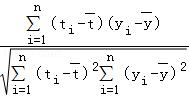
\includegraphics[width=.38\linewidth]{question-18-1.jpg}
\end{center}
\begin{solution}
\textbf{答案：}见解析

\textbf{分析：}(1) 由折线图看出, $y$ 与 $t$ 之间存在较强的正相关关系, 将已知数据代入相关系数方程, 可得答案; (2) 根据已知中的数据, 求出回归系数, 可得回归方程, $2016$ 年对应的 $t$ 值为 $9$, 代入可预测 $2016$ 年我国生活垃圾无害化处理量.

\textbf{详解：}(Ⅰ) 由折线图得 $\bar{t}=\frac{1+2+\cdots+7}{7}=4$, $\sum_{i=1}^{7}(t_i-\bar{t})^2=28$. $\sum_{i=1}^{7}(t_i-\bar{t})(y_i-\bar{y})=\sum_{i=1}^{7}t_iy_i-\bar{t}\sum_{i=1}^{7}y_i=40.17-4\times9.32=40.17-37.28=2.89$. $\sqrt{\sum_{i=1}^{7}(y_i-\bar{y})^2}=0.55$, $\sqrt{\sum_{i=1}^{7}(t_i-\bar{t})^2}=\sqrt{28}=2\sqrt{7}\approx2\times2.646=5.292$. 所以 $r=\dfrac{2.89}{5.292\times0.55}\approx\dfrac{2.89}{2.9106}\approx0.993$. 因为 $0.993>0.75$, 故 $y$ 与 $t$ 之间存在较强的正相关关系.
(Ⅱ) $\hat{b}=\dfrac{2.89}{28}\approx0.103$, $\bar{y}=\dfrac{9.32}{7}\approx1.331$, $\hat{a}=\bar{y}-\hat{b}\bar{t}\approx1.331-0.103\times4=0.92$. 所以 $y$ 关于 $t$ 的回归方程为 $\hat{y}=0.10t+0.92$. $2016$ 年对应的 $t=9$, 代入得 $\hat{y}=0.10\times9+0.92=1.82$. 所以预测 $2016$ 年我国生活垃圾无害化处理量为 $1.82$ 亿吨.
\end{solution}
\end{question}

\begin{question}[points=12]
如图, 四棱锥 $P-ABCD$ 中, $PA\perp$ 底面 $ABCD$, $AD\parallel BC$, $AB=AD=AC=3$, $PA=BC=4$, $M$ 为线段 $AD$ 上一点, $AM=2MD$, $N$ 为 $PC$ 的中点.

(Ⅰ) 证明 $MN\parallel$ 平面 $PAB$;

(Ⅱ) 求四面体 $N-BCM$ 的体积.

\begin{center}
  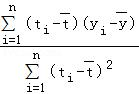
\includegraphics[width=.38\linewidth]{question-19-1.jpg}
\end{center}
\begin{solution}
\textbf{答案：}见解析

\textbf{分析：}(Ⅰ) 取 $BC$ 中点 $E$, 连结 $EN$, $EM$, 得 $NE$ 是 $\triangle PBC$ 的中位线, 推导出四边形 $ABEM$ 是平行四边形, 由此能证明 $MN\parallel$ 平面 $PAB$.
(Ⅱ) 取 $AC$ 中点 $F$, 连结 $NF$, $NF$ 是 $\triangle PAC$ 的中位线, 推导出 $NF\perp$ 面 $ABCD$, 延长 $BC$ 至 $G$, 使得 $CG=AM$, 连结 $GM$, 则四边形 $AGCM$ 是平行四边形, 由此能求出四面体 $N-BCM$ 的体积.

\textbf{详解：}(Ⅰ) 取 $BC$ 中点 $E$, 连结 $EN$, $EM$. 因为 $N$ 为 $PC$ 的中点, 所以 $NE$ 是 $\triangle PBC$ 的中位线, 所以 $NE\parallel PB$. 又 $AD\parallel BC$, 所以 $BE\parallel AD$. 因为 $AB=AD=AC=3$, $PA=BC=4$, $AM=2MD$, 所以 $BE=\dfrac{1}{2}BC=2=AM$, 所以四边形 $ABEM$ 是平行四边形, 所以 $EM\parallel AB$. 所以平面 $NEM\parallel$ 平面 $PAB$. 因为 $MN\subset$ 平面 $NEM$, 所以 $MN\parallel$ 平面 $PAB$.
(Ⅱ) 取 $AC$ 中点 $F$, 连结 $NF$. 因为 $NF$ 是 $\triangle PAC$ 的中位线, 所以 $NF\parallel PA$, $NF=\dfrac{1}{2}PA=2$. 又 $PA\perp$ 面 $ABCD$, 所以 $NF\perp$ 面 $ABCD$. 延长 $BC$ 至 $G$, 使得 $CG=AM$, 连结 $GM$. 因为 $AM\parallel CG$, 所以四边形 $AGCM$ 是平行四边形, 所以 $AC=MG=3$. 又 $ME=3$, $EC=CG=2$, 所以 $\triangle MEG$ 的高 $h=\sqrt{3^2-(\frac{4}{2})^2}=\sqrt{5}$, 所以 $S_{\triangle BCM}=\dfrac{1}{2}\times BC\times h=\dfrac{1}{2}\times4\times\sqrt{5}=2\sqrt{5}$. 所以四面体 $N-BCM$ 的体积 $V_{N-BCM}=\dfrac{1}{3}\times NF\times S_{\triangle BCM}=\dfrac{1}{3}\times2\times2\sqrt{5}=\dfrac{4\sqrt{5}}{3}$.
\end{solution}
\end{question}

\begin{question}[points=12]
已知抛物线 $C: y^2=2x$ 的焦点为 $F$, 平行于 $x$ 轴的两条直线 $l_1$, $l_2$ 分别交 $C$ 于 $A$, $B$ 两点, 交 $C$ 的准线于 $P$, $Q$ 两点.

(Ⅰ) 若 $F$ 在线段 $AB$ 上, $R$ 是 $PQ$ 的中点, 证明 $AR\parallel FQ$;

(Ⅱ) 若 $\triangle PQF$ 的面积是 $\triangle ABF$ 的面积的两倍, 求 $AB$ 中点的轨迹方程.
\begin{solution}
\textbf{答案：}见解析

\textbf{分析：}(Ⅰ) 连接 $RF$, $PF$, 利用等角的余角相等, 证明 $\angle PRA=\angle PQF$, 即可证明 $AR\parallel FQ$;
(Ⅱ) 利用 $\triangle PQF$ 的面积是 $\triangle ABF$ 的面积的两倍, 求出 $N$ 的坐标, 利用点差法求 $AB$ 中点的轨迹方程.

\textbf{详解：}(Ⅰ) 连接 $RF$, $PF$. 由 $AP=AF$, $BQ=BF$ 及 $AP\parallel BQ$, 得 $\angle AFP+\angle BFQ=90^{\circ}$, 所以 $\angle PFQ=90^{\circ}$. 因为 $R$ 是 $PQ$ 的中点, 所以 $RF=RP=RQ$, 所以 $\triangle PAR\cong\triangle FAR$, 所以 $\angle PAR=\angle FAR$, $\angle PRA=\angle FRA$. 又 $\angle BQF+\angle BFQ=180^{\circ}-\angle QBF=\angle PAF=2\angle PAR$, 所以 $\angle FQB=\angle PAR$, 所以 $\angle PRA=\angle PQF$, 所以 $AR\parallel FQ$.
(Ⅱ) 设 $A(x_1,y_1)$, $B(x_2,y_2)$, $F(\frac{1}{2},0)$, 准线为 $x=-\frac{1}{2}$. $S_{\triangle PQF}=\frac{1}{2}|PQ|=\frac{1}{2}|y_1-y_2|$. 设直线 $AB$ 与 $x$ 轴交点为 $N$, 则 $S_{\triangle ABF}=\frac{1}{2}|FN||y_1-y_2|$. 因为 $\triangle PQF$ 的面积是 $\triangle ABF$ 的面积的两倍, 所以 $2|FN|=1$, 得 $x_N=1$, 即 $N(1,0)$. 设 $AB$ 中点为 $M(x,y)$, 由 $\begin{cases}y_1^2=2x_1\\ y_2^2=2x_2\end{cases}$ 得 $(y_1-y_2)(y_1+y_2)=2(x_1-x_2)$, 又 $\dfrac{y_1-y_2}{x_1-x_2}=\dfrac{y}{x-1}$, 所以 $y\cdot2y=2$, 即 $y^2=x-1$. 所以 $AB$ 中点轨迹方程为 $y^2=x-1$.
\end{solution}
\end{question}

\begin{question}[points=12]
设函数 $f(x)=\ln x-x+1$.

(1) 讨论 $f(x)$ 的单调性;

(2) 证明当 $x\in(1,+\infty)$ 时, $1<\dfrac{x-1}{\ln x}<x$;

(3) 设 $c>1$, 证明当 $x\in(0,1)$ 时, $1+(c-1)x>c^x$.
\begin{solution}
\textbf{答案：}见解析

\textbf{分析：}(1) 求出导数, 由导数大于0可得增区间, 导数小于0可得减区间, 注意函数的定义域;
(2) 由题意可得即证 $\ln x<x-1<x\ln x$. 运用(1)的单调性可得 $\ln x<x-1$, 设 $F(x)=x\ln x-x+1$, $x>1$, 求出单调性, 即可得到 $x-1<x\ln x$ 成立;
(3) 设 $G(x)=1+(c-1)x-c^x$, 求 $G(x)$ 的二次导数, 判断 $G'(x)$ 的单调性, 进而证明原不等式.

\textbf{详解：}(1) $f(x)=\ln x-x+1$, $f'(x)=\frac{1}{x}-1=\frac{1-x}{x}$, $x>0$. 由 $f'(x)>0$ 得 $0<x<1$, 由 $f'(x)<0$ 得 $x>1$. 所以 $f(x)$ 的增区间为 $(0,1)$, 减区间为 $(1,+\infty)$.
(2) 当 $x>1$ 时, $1<\frac{x-1}{\ln x}<x$ 等价于 $\ln x<x-1<x\ln x$. 由(1)知 $f(x)=\ln x-x+1$ 在 $(1,+\infty)$ 递减, 所以 $f(x)<f(1)=0$, 即 $\ln x<x-1$. 设 $F(x)=x\ln x-x+1$, $x>1$, 则 $F'(x)=\ln x+1-1=\ln x>0$, 所以 $F(x)$ 在 $(1,+\infty)$ 递增, 所以 $F(x)>F(1)=0$, 即 $x\ln x>x-1$. 故原不等式成立.
(3) 设 $G(x)=1+(c-1)x-c^x$, $x\in(0,1)$, $c>1$. 则 $G'(x)=c-1-c^x\ln c$, $G''(x)=-(\ln c)^2 c^x<0$, 所以 $G'(x)$ 在 $(0,1)$ 单调递减. $G'(0)=c-1-\ln c$, $G'(1)=c-1-c\ln c$. 由(1)知 $f(x)=\ln x-x+1$, 当 $x=c$ 时, $f(c)=\ln c-c+1<0$, 所以 $c-1-\ln c>0$, 即 $G'(0)>0$. 由(2)知 $\frac{x-1}{\ln x}<x$, 取 $x=c$ 得 $\frac{c-1}{\ln c}<c$, 即 $c-1<c\ln c$, 所以 $G'(1)=c-1-c\ln c<0$. 故存在 $t\in(0,1)$ 使得 $G'(t)=0$. 所以 $x\in(0,t)$ 时 $G'(x)>0$, $x\in(t,1)$ 时 $G'(x)<0$, 即 $G(x)$ 在 $(0,t)$ 递增, 在 $(t,1)$ 递减. 又 $G(0)=1+0-1=0$, $G(1)=1+(c-1)-c=0$, 所以 $x\in(0,1)$ 时 $G(x)>0$ 成立, 即 $1+(c-1)x>c^x$.
\end{solution}
\end{question}

\section*{选做题}
请考生在第22-24题中任选一题做答, 如果多做, 则按所做的第一题计分.

\begin{question}[points=10]
如图, $\odot O$ 中 $\widehat{AB}$ 的中点为 $P$, 弦 $PC$, $PD$ 分别交 $AB$ 于 $E$, $F$ 两点.

(1) 若 $\angle PFB=2\angle PCD$, 求 $\angle PCD$ 的大小;

(2) 若 $EC$ 的垂直平分线与 $FD$ 的垂直平分线交于点 $G$, 证明: $OG\perp CD$.

\begin{center}
  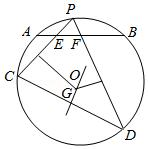
\includegraphics[width=.38\linewidth]{question-22-1.jpg}
\end{center}
\begin{solution}
\textbf{答案：}见解析

\textbf{分析：}(1) 连接 $PA$, $PB$, $BC$, 设 $\angle PEB=\angle1$, $\angle PCB=\angle2$, $\angle ABC=\angle3$, $\angle PBA=\angle4$, $\angle PAB=\angle5$, 运用圆的性质和四点共圆的判断, 可得 $E$, $C$, $D$, $F$ 共圆, 再由圆内接四边形的性质, 即可得到所求 $\angle PCD$ 的度数;
(2) 运用圆的定义和 $E$, $C$, $D$, $F$ 共圆, 可得 $G$ 为圆心, $G$ 在 $CD$ 的中垂线上, 即可得证.

\textbf{详解：}(1) 连接 $PB$, $BC$. 设 $\angle PEB=\angle1$, $\angle PCB=\angle2$, $\angle ABC=\angle3$, $\angle PBA=\angle4$, $\angle PAB=\angle5$. 由 $\odot O$ 中 $\widehat{AB}$ 的中点为 $P$, 可得 $\angle4=\angle5$. 在 $\triangle EBC$ 中, $\angle1=\angle2+\angle3$, 又 $\angle D=\angle3+\angle4$, $\angle2=\angle5$, 所以 $\angle2=\angle4$, 则 $\angle D=\angle1$. 故 $E$, $C$, $D$, $F$ 四点共圆, 所以 $\angle EFD+\angle PCD=180^{\circ}$. 由 $\angle PFB=\angle EFD=2\angle PCD$ 得 $3\angle PCD=180^{\circ}$, 所以 $\angle PCD=60^{\circ}$.
(2) 由 $C$, $D$, $E$, $F$ 四点共圆, $EC$ 的垂直平分线与 $FD$ 的垂直平分线交于点 $G$, 可得 $G$ 为圆心, 所以 $GC=GD$. 故 $G$ 在 $CD$ 的中垂线上. 又 $CD$ 为圆 $G$ 的弦, 所以 $OG\perp CD$.
\end{solution}
\end{question}

\begin{question}[points=10]
在直角坐标系 $xOy$ 中, 曲线 $C_1$ 的参数方程为 $\begin{cases}x=\sqrt{3}\cos\alpha\\ y=\sin\alpha\end{cases}$ ($\alpha$ 为参数), 以坐标原点为极点, 以 $x$ 轴的正半轴为极轴, 建立极坐标系, 曲线 $C_2$ 的极坐标方程为 $\rho\sin(\theta+\frac{\pi}{4})=2\sqrt{2}$.

(1) 写出 $C_1$ 的普通方程和 $C_2$ 的直角坐标方程;

(2) 设点 $P$ 在 $C_1$ 上, 点 $Q$ 在 $C_2$ 上, 求 $|PQ|$ 的最小值及此时 $P$ 的直角坐标.
\begin{solution}
\textbf{答案：}见解析

\textbf{分析：}(1) 运用两边平方和同角的平方关系, 即可得到 $C_1$ 的普通方程, 运用 $x=\rho\cos\theta$, $y=\rho\sin\theta$, 以及两角和的正弦公式, 化简可得 $C_2$ 的直角坐标方程;
(2) 由题意可得当直线 $x+y-4=0$ 的平行线与椭圆相切时, $|PQ|$ 取得最值. 设与直线 $x+y-4=0$ 平行的直线方程为 $x+y+t=0$, 代入椭圆方程, 运用判别式为 $0$, 求得 $t$, 再由平行线的距离公式, 可得 $|PQ|$ 的最小值, 解方程可得 $P$ 的直角坐标. 另解: 设 $P(\sqrt{3}\cos\alpha,\sin\alpha)$, 由点到直线的距离公式, 结合辅助角公式和正弦函数的值域, 即可得到所求最小值和 $P$ 的坐标.

\textbf{详解：}(1) $C_1$: $\begin{cases}x=\sqrt{3}\cos\alpha\\ y=\sin\alpha\end{cases}$, 消去参数得 $\dfrac{x^2}{3}+y^2=1$. $C_2$: $\rho\sin(\theta+\frac{\pi}{4})=2\sqrt{2}$, 即 $\rho(\frac{\sqrt{2}}{2}\sin\theta+\frac{\sqrt{2}}{2}\cos\theta)=2\sqrt{2}$, 所以 $\rho\sin\theta+\rho\cos\theta=4$, 由 $x=\rho\cos\theta$, $y=\rho\sin\theta$ 得 $x+y-4=0$.
(2) 设与直线 $x+y-4=0$ 平行的直线为 $x+y+t=0$, 代入 $\dfrac{x^2}{3}+y^2=1$ 得 $4x^2+6tx+3t^2-3=0$. 由 $\Delta=36t^2-16(3t^2-3)=0$ 得 $t=\pm2$. 当 $t=-2$ 时, $|PQ|$ 取得最小值, $|PQ|=\dfrac{|-2-(-4)|}{\sqrt{2}}=\sqrt{2}$. 此时 $4x^2-12x+9=0$, 解得 $x=\frac{3}{2}$, $y=-x-2=-\frac{3}{2}-2=-\frac{1}{2}$, 所以 $P(\frac{3}{2},-\frac{1}{2})$.
另解: 设 $P(\sqrt{3}\cos\alpha,\sin\alpha)$, 则 $P$ 到直线 $x+y-4=0$ 的距离 $d=\dfrac{|\sqrt{3}\cos\alpha+\sin\alpha-4|}{\sqrt{2}}=\dfrac{|2\sin(\alpha+\frac{\pi}{3})-4|}{\sqrt{2}}$, 当 $\sin(\alpha+\frac{\pi}{3})=1$ 时, $d$ 最小, 最小值为 $\dfrac{|-2|}{\sqrt{2}}=\sqrt{2}$, 此时 $\alpha+\frac{\pi}{3}=2k\pi+\frac{\pi}{2}$, 取 $\alpha=\frac{\pi}{6}$, 则 $P(\frac{3}{2},\frac{1}{2})$.
\end{solution}
\end{question}

\begin{question}[points=10]
已知函数 $f(x)=|2x-a|+a$.

(1) 当 $a=2$ 时, 求不等式 $f(x)\le 6$ 的解集;

(2) 设函数 $g(x)=|2x-1|$, 当 $x\in\mathbb{R}$ 时, $f(x)+g(x)\ge 3$, 求 $a$ 的取值范围.
\begin{solution}
\textbf{答案：}见解析

\textbf{分析：}(1) 当 $a=2$ 时, 由已知得 $|2x-2|+2\le 6$, 由此能求出不等式 $f(x)\le 6$ 的解集.
(2) 由 $f(x)+g(x)=|2x-1|+|2x-a|+a\ge 3$, 得 $|x-\frac{1}{2}|+|x-\frac{a}{2}|\ge \frac{3-a}{2}$, 由此能求出 $a$ 的取值范围.

\textbf{详解：}(1) 当 $a=2$ 时, $f(x)=|2x-2|+2$, $f(x)\le 6$ 即 $|2x-2|+2\le 6$, $|2x-2|\le 4$, $|x-1|\le 2$, $-2\le x-1\le 2$, 解得 $-1\le x\le 3$. 所以不等式的解集为 $\{x|-1\le x\le 3\}$.
(2) $f(x)+g(x)=|2x-1|+|2x-a|+a\ge 3$ 即 $2|x-\frac{1}{2}|+2|x-\frac{a}{2}|+a\ge 3$, $|x-\frac{1}{2}|+|x-\frac{a}{2}|\ge \frac{3-a}{2}$. 当 $a\ge 3$ 时, 右边 $\le 0$, 不等式恒成立. 当 $a<3$ 时, 左边最小值 $\frac{1}{2}|a-1|\ge \frac{3-a}{2}$ $>0$, 平方得 $(a-1)^2\ge (3-a)^2$, 解得 $a\ge 2$, 所以 $2\le a<3$. 综上, $a$ 的取值范围是 $[2,+\infty)$.
\end{solution}
\end{question}

